\section{Estrategias de la Organización }
\section{Estructura Organizacional en el área de TI}

%%%%%%%%%%%%%%%%%%%%%%%%%%%%%%%%%%%%%%%%%%%%%%%%%%%%%%%%%%%%%%%%%%%%%%%%%%%%%%%%%
%	                   Políticas de TI 
%%%%%%%%%%%%%%%%%%%%%%%%%%%%%%%%%%%%%%%%%%%%%%%%%%%%%%%%%%%%%%%%%%%%%%%%%%%%%%%%%

\subsection{Políticas de TI}
    \begin{figure}[!ht]
        \centering
        \href{https://klintex.com.pe/wp-content/uploads/2021/12/Politica-Privacidad_-Klintex.pdf}{
                
\includegraphics[width=0.25\textwidth]{icon_pdf.png}
                }
    \end{figure}    
%%%%%%%%%%%%%%%%%%%%%%%%%%%%%%%%%%%%%%%%%%%%%%%%%%%%%%%%%%%%%%%%%%%%%%%%%%%%%%%%%
%	                   Objetivos de TI 
%%%%%%%%%%%%%%%%%%%%%%%%%%%%%%%%%%%%%%%%%%%%%%%%%%%%%%%%%%%%%%%%%%%%%%%%%%%%%%%%%

\subsection{Objetivos de TI}
    \begin{itemize}
        \item Completar la migración de la empresa de logística en El Salvador de SAP ERP (ECC 6.0) a SAP S/4HANA, asegurando una integración sin fisuras y la eliminación de problemas de transferencia de datos entre sistemas. 
        \item Actualizar las APIs utilizadas en el módulo de gestión de la cadena de suministro (SCM) para mejorar la sincronización de datos en tiempo real y reducir los retrasos en la gestión de pedidos, aumentando la eficiencia operativa. 
        \item Aumentar el ancho de banda de la red en El Salvador y actualizar los routers a equipos más modernos, como los Cisco ISR 4000, para reducir la latencia y mejorar la estabilidad y capacidad de la red durante horas pico. 
        \item Migrar de un sistema de sincronización de datos batch a uno en tiempo real para procesos críticos de la cadena de suministro y logística, garantizando la actualización instantánea de pedidos y el estado de inventarios. 
        \item Implementar un sistema de monitoreo continuo para detectar y resolver proactivamente problemas de sincronización de datos y de red, minimizando el impacto en las operaciones logísticas. 
        \item Desarrollar un equipo de soporte técnico especializado en El Salvador, capacitado para resolver de manera rápida y eficiente cualquier problema relacionado con TI y la infraestructura de red, asegurando la continuidad del servicio. 
        \item Optimizar la red VPN privada utilizada en El Salvador para reducir la latencia a menos de 150 ms durante horas pico y garantizar un ancho de banda suficiente para soportar las operaciones críticas de logística. 
        \item Desarrollar e implementar un plan de contingencia robusto que permita a Alicorp mantener la continuidad operativa en El Salvador frente a posibles interrupciones en la red o fallas en el sistema, minimizando el impacto en la cadena de suministro y la satisfacción del cliente.
    \end{itemize}
\subsection{Organización del área de TI}
    \begin{figure}[!ht]
        \centering
        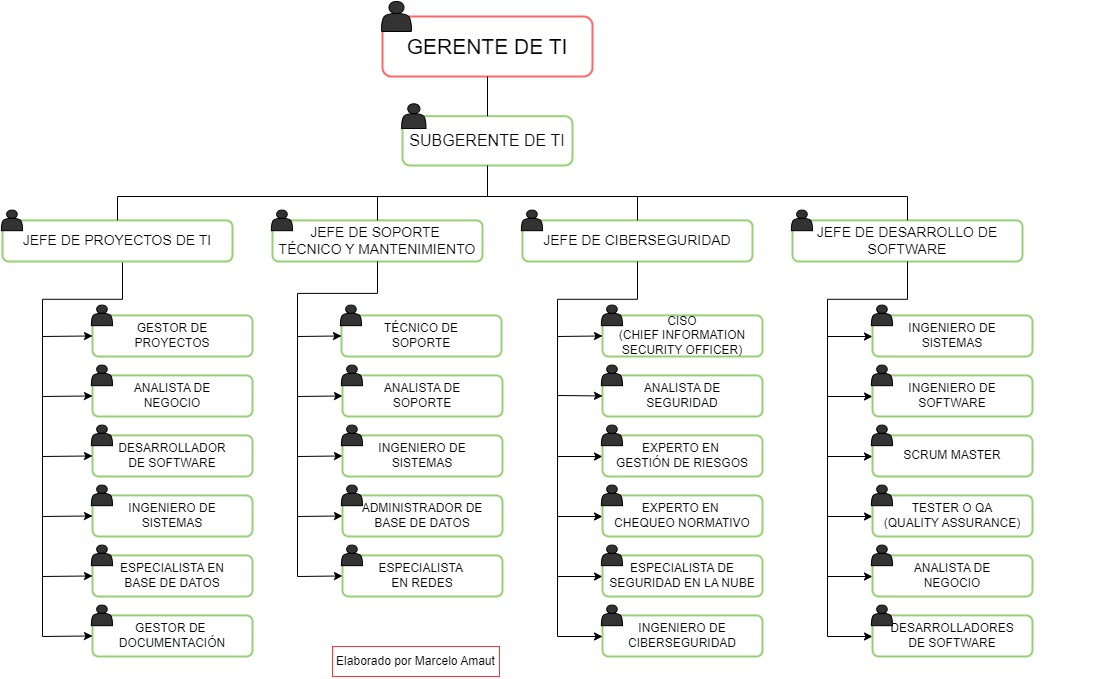
\includegraphics[width=0.8\textwidth]{estructura_organizacional_alicorp.jpeg}
        \caption{Organigrama  de la organización del área de TI}
    \end{figure}

%%%%%%%%%%%%%%%%%%%%%%%%%%%%%%%%%%%%%%%%%%%%%%%%%%%%%%%%%%%%%%%%%%%%%%%%%%%%%%%%%
%	                   Descripción de las áreas de TI
%%%%%%%%%%%%%%%%%%%%%%%%%%%%%%%%%%%%%%%%%%%%%%%%%%%%%%%%%%%%%%%%%%%%%%%%%%%%%%%%%

\subsection{Descripción de las áreas de TI}
    \subsubsection{Área de TI}
    El área de TI en Alicorp es el pilar tecnológico que impulsa la eficiencia y la innovación en la empresa. Su rol principal es diseñar, implementar y mantener la infraestructura tecnológica necesaria para las operaciones diarias. Esto incluye desde la gestión de redes y servidores hasta el desarrollo de software a medida y el análisis de grandes volúmenes de datos. 
    La TI en Alicorp es mucho más que un simple departamento de soporte. Es un socio estratégico que contribuye al éxito de la empresa de diversas maneras. Automatiza procesos, mejora la toma de decisiones, optimiza la cadena de suministro y fortalece la relación con los clientes. Además, fomenta una cultura de innovación constante, explorando nuevas tecnologías y tendencias del mercado. 
    \subsubsection{Área de Infraestructura de TI}
    El Área de Infraestructura de TI en Alicorp es la base sobre la cual se construye toda la operación tecnológica de la empresa. Es la división encargada de diseñar, implementar y mantener la red de sistemas, servidores, almacenamiento de datos y demás componentes hardware que permiten el funcionamiento óptimo de las aplicaciones y servicios de la compañía. 
    La infraestructura de TI es como el esqueleto de un cuerpo humano. Mientras que las aplicaciones y software son los órganos que permiten realizar las tareas, la infraestructura es la estructura que los sostiene y conecta. En Alicorp, esta área se encarga de que todos los componentes tecnológicos trabajen en conjunto de manera eficiente y segura. 
    \subsubsection{Área de proyectos de TI}
    El Área de Proyectos de TI en Alicorp es el corazón pulsante de la transformación digital de la empresa. Es el equipo encargado de concebir, planificar y ejecutar iniciativas tecnológicas que buscan optimizar procesos, mejorar la eficiencia y generar valor para el negocio. 
    El área de proyectos de TI se puede visualizar como un taller de construcción. Mientras que la infraestructura es el edificio, los proyectos son las reformas y ampliaciones que lo modernizan y adaptan a las nuevas necesidades. Estos proyectos pueden ir desde la implementación de un nuevo sistema de gestión de inventario hasta el desarrollo de una plataforma de comercio electrónico. 
    Para llevar a cabo sus proyectos, el área de proyectos de TI en Alicorp utiliza metodologías ágiles como Scrum o Kanban. Estas metodologías permiten una mayor flexibilidad, adaptabilidad y colaboración entre los equipos, lo que facilita la entrega de valor de manera incremental. 
    \subsubsection{Área de mantenimiento: }
    El área de mantenimiento de software en Alicorp es el equipo encargado de asegurar que todas las aplicaciones y sistemas informáticos de la empresa funcionen de manera correcta y eficiente. Es como un equipo de médicos especializados en tecnología, que diagnostican, tratan y previenen "enfermedades" en el software. 
    Imaginemos el software como un automóvil. Al igual que un auto necesita revisiones periódicas y reparaciones para mantenerlo en buen estado, las aplicaciones de Alicorp también requieren de un mantenimiento constante. El equipo de mantenimiento de software se encarga de realizar estas revisiones, solucionar problemas y actualizar el software para adaptarlo a las nuevas necesidades del negocio. 
    Las principales funciones del área de mantenimiento de software radican en la corrección de errores, donde se identifica y soluciona los errores o bugs que puedan surgir en las aplicaciones, evitando que afecten el funcionamiento normal del sistema. También están las actualizaciones, es decir, los parches de seguridad y actualizaciones para mejorar el rendimiento y la seguridad del software. Además, se trabaja con una cultura de mejora continua, realizando mejoras en las aplicaciones para aumentar su eficiencia y funcionalidad. 
    Es importante utilizar herramientas y metodologías para llevar estas funciones, por eso existe un sistema de control de versiones que permiten gestionar los cambios en el código fuente de las aplicaciones y entornos de desarrollo integrados que facilitan la programación y depuración de código. Por último, es necesario hablar de las herramientas de automatización, tales como scripts y programas que automatizan tareas repetitivas, como la generación de informes o la ejecución de pruebas. 

%%%%%%%%%%%%%%%%%%%%%%%%%%%%%%%%%%%%%%%%%%%%%%%%%%%%%%%%%%%%%%%%%%%%%%%%%%%%%%%%%
%	                   CIO 
%%%%%%%%%%%%%%%%%%%%%%%%%%%%%%%%%%%%%%%%%%%%%%%%%%%%%%%%%%%%%%%%%%%%%%%%%%%%%%%%%

\subsection{CIO}
    \subsubsection{Funciones}
        \begin{itemize}
            \item Gestionar el personal del área de informática. 
            \item Negociar las relaciones con los proveedores. 
            \item Supervisar la arquitectura de TI. 
            \item Definir las políticas, normas y procesos de gobernanza de las TI. 
            \item Gestionar el riesgo de la información. 
            \item Tomar decisiones sobre el gasto e inversión en TI. 
            \item Gestionar la capacidad y el ciclo de vida de la tecnología. 
            \item Comprender las tendencias tecnológicas y su aplicabilidad a los objetivos de la empresa. 
            \item Comunicar la gestión de incidentes importantes a los ejecutivos y otras partes interesadas. 
            \item Encargarse del cumplimiento de normativas gubernamentales en materia de TI 
        \end{itemize}

    \subsubsection{Responsabilidades }
        \begin{itemize}
            \item Impulsar la innovación tecnológica dentro del sector en el que se desenvuelve la compañía. 
            \item Asegurar el funcionamiento continuo y el rendimiento óptimo de las plataformas y sistemas esenciales para la operación del negocio. 
            \item Trabajar de manera conjunta con los equipos de desarrollo y operaciones para garantizar la implementación puntual de soluciones tecnológicas. 
            \item Supervisar la formación y el crecimiento profesional del equipo de tecnología. 
            \item Identificar y mitigar los riesgos asociados con la seguridad de la información y los sistemas tecnológicos. 
            \item Forjar relaciones estratégicas con proveedores clave de tecnología y servicios. 
            \item Contribuir en la planificación financiera y el control de gastos en el área tecnológica. 
            \item Comunicar de forma clara y efectiva la estrategia tecnológica y los avances logrados a las partes interesadas tanto internas como externas. 
            \item Analizar cómo la tecnología influye en la productividad y eficiencia de la empresa, sugiriendo mejoras de manera constante. 
        \end{itemize}

    \subsubsection{Perfil de un CIO}
    El perfil de un CIO (Chief Information Officer) en una organización de gran tamaño debe reunir una sólida formación en tecnologías de la información, una visión estratégica clara y habilidades de liderazgo excepcionales. Este ejecutivo debe contar con una experiencia comprobada en la implementación de soluciones tecnológicas innovadoras que optimicen los procesos operativos y faciliten la transformación digital de la empresa. Además, es esencial que tenga la capacidad de liderar equipos multidisciplinarios, manejar proyectos tecnológicos complejos y comunicarse eficazmente con las diferentes partes involucradas. 
    El CIO debe estar preparado para identificar y adoptar nuevas tecnologías de manera proactiva, que impulsen la eficiencia y competitividad de la compañía, garantizando al mismo tiempo la seguridad de la información y el cumplimiento de las normativas vigentes. También es crucial que mantenga una mentalidad estratégica que asegure la alineación de la tecnología con los objetivos corporativos, así como la creación de alianzas estratégicas con proveedores y socios clave. En resumen, el CIO ideal debe ser un líder visionario, con una sólida formación técnica y una clara orientación hacia la innovación y la eficiencia en la implementación de soluciones tecnológicas. 
        \paragraph*{Especificaciones del Perfil }
        \begin{itemize}
            \item Experiencia previa en la implementación de soluciones tecnológicas en la industria de consumo masivo, debe haber liderado proyectos exitosos en la implementación de tecnología para optimizar la cadena de suministro, la producción y la distribución de productos en empresas de gran escala. Es esencial tener un historial comprobado en la mejora de procesos logísticos, automatización de plantas y sistemas de distribución. 
            \item Conocimiento profundo de las tecnologías de la información aplicadas a la producción y logística, debe estar familiarizado con tecnologías como IoT, automatización industrial, inteligencia artificial y análisis de datos, plataformas de gestión de inventario y logística, así como sistemas ERP y CRM utilizados en la industria de consumo masivo. 
            \item Habilidades de liderazgo comprobadas en entornos complejos y de alto rendimiento, debe ser capaz de liderar equipos multidisciplinarios que incluyan profesionales de TI, ingeniería, y operaciones, creando un ambiente colaborativo y orientado a resultados dentro de una industria que opera a gran escala. 
            \item Experiencia en la gestión de la seguridad de la información y protección de datos en un entorno de operaciones complejas, asegurar el cumplimiento de las normativas de seguridad de la información y la protección de datos, en especial en la privacidad del cliente y la integridad de los sistemas de producción y distribución. 
            \item Capacidad para desarrollar e implementar estrategias tecnológicas alineadas con los objetivos de crecimiento de la empresa, debe ser capaz de impulsar la innovación tecnológica que mejore la eficiencia de la producción y la distribución, optimizando procesos operativos y mejorando la agilidad en la respuesta a las demandas del mercado. 
            \item Excelentes habilidades de comunicación, es crucial que pueda colaborar eficazmente con otros líderes empresariales dentro de la organización, como las áreas de operaciones, finanzas y marketing, así como interactuar con socios estratégicos y proveedores clave en el sector de tecnología. 
            \item Experiencia en la gestión de proyectos tecnológicos complejos dentro del sector de alimentos y productos de consumo masivo: El CIO debe asegurar que los proyectos tecnológicos, como la modernización de plantas de producción o la implementación de sistemas logísticos, se entreguen a tiempo y dentro del presupuesto. 
            \item Visión estratégica para identificar oportunidades de crecimiento y optimización tecnológica: Debe poder proponer y liderar iniciativas tecnológicas que maximicen la eficiencia y el crecimiento del negocio, centrando en la sostenibilidad y la innovación en la producción y distribución de productos. 
            \item Entendimiento profundo de los desafíos del sector de consumo masivo: El CIO debe estar familiarizado con las particularidades del mercado, las tendencias de consumo y los desafíos que enfrenta una empresa de la escala de Alicorp, siendo capaz de ofrecer soluciones tecnológicas que potencien su competitividad y liderazgo en el mercado. 
        \end{itemize}
%%%%%%%%%%%%%%%%%%%%%%%%%%%%%%%%%%%%%%%%%%%%%%%%%%%%%%%%%%%%%%%%%%%%%%%%%%%%%%%%%
%	                  Diagnóstico de la Situación Actual de las TICS 
%%%%%%%%%%%%%%%%%%%%%%%%%%%%%%%%%%%%%%%%%%%%%%%%%%%%%%%%%%%%%%%%%%%%%%%%%%%%%%%%%


\subsection{Diagnóstico de la Situación Actual de las TICS}
    \subsubsection{Capacidades de las TIC’s }
    Basándonos en la información disponible, podemos inferir que Alicorp ha desarrollado un sólido ecosistema tecnológico, destacando en las siguientes áreas: 

        \paragraph*{Gestión de la Cadena de Suministro} 
        Alicorp ha invertido significativamente en la implementación de sistemas ERP (Enterprise Resource Planning) que integran y automatizan diversas funciones de la cadena de suministro, desde la planificación de la producción hasta la gestión de inventario y la distribución. Estos sistemas permiten a la empresa: 
        Optimizar la planificación de la producción: Al contar con datos precisos sobre la demanda y el inventario, Alicorp puede ajustar su producción de manera más eficiente, evitando sobrestocks y faltantes. 
        Mejorar la gestión de inventario: Los sistemas ERP permiten un seguimiento en tiempo real del inventario, lo que reduce los costos asociados a la sobreproducción o a la falta de stock. 
        Optimizar las rutas de distribución: Mediante el uso de herramientas de análisis de datos y algoritmos de optimización, Alicorp puede planificar las rutas de distribución de manera más eficiente, reduciendo costos y tiempos de entrega. 
        Aumentar la visibilidad de la cadena de suministro: El IoT (Internet de las Cosas) juega un papel fundamental al permitir el seguimiento en tiempo real de los productos a lo largo de toda la cadena de suministro, desde la materia prima hasta el consumidor final. Esto facilita la identificación de posibles problemas y la toma de decisiones más ágiles. 

        \paragraph*{Producción}
        La aplicación de las TICs en los procesos productivos de Alicorp ha permitido mejorar significativamente la eficiencia y la calidad. Algunos ejemplos son: 
        Automatización de procesos: La implementación de robots y sistemas automatizados en las líneas de producción ha reducido los errores humanos, aumentado la productividad y mejorado la seguridad de los trabajadores. 
        Control de calidad: El uso de sensores y sistemas de monitoreo en tiempo real permite detectar y corregir cualquier desviación de los estándares de calidad de manera temprana. 
        Simulación de procesos: Las herramientas de simulación permiten evaluar diferentes escenarios y optimizar los procesos productivos antes de implementarlos en la realidad, reduciendo costos y tiempo de puesta en marcha. 
    
        \paragraph*{Ventas y Marketing} 
        Alicorp ha adoptado una estrategia de marketing digital y análisis de datos para conocer mejor a sus consumidores y ofrecerles productos y servicios más personalizados. Esto se traduce en: 
        Análisis de datos: La recopilación y análisis de grandes volúmenes de datos sobre los consumidores permite identificar patrones de comportamiento, preferencias y tendencias. 
        Personalización de la experiencia del cliente: Gracias al análisis de datos, Alicorp puede ofrecer recomendaciones de productos personalizadas, campañas de marketing segmentadas y experiencias de compra más relevantes. 
        Comercio electrónico: La empresa ha desarrollado plataformas de comercio electrónico que permiten a los consumidores adquirir sus productos de manera fácil y rápida, con opciones de pago y entrega flexibles. 
        Marketing digital: Alicorp utiliza una amplia variedad de canales digitales, como redes sociales, motores de búsqueda y email marketing, para llegar a su público objetivo y generar engagement. 
    
        \paragraph*{Investigación y Desarrollo}
        Las TICs también están desempeñando un papel clave en la investigación y desarrollo de nuevos productos en Alicorp. Algunas de las aplicaciones más destacadas son: 
        Diseño asistido por computadora (CAD): El uso de software CAD permite a los ingenieros diseñar nuevos productos de manera más rápida y precisa, reduciendo los tiempos de desarrollo. 
        Simulación: Las herramientas de simulación permiten evaluar el desempeño de los nuevos productos en diferentes condiciones, lo que facilita la identificación de posibles problemas y la optimización del diseño. 
        Análisis de datos: El análisis de datos provenientes de la investigación de mercado y de los consumidores permite identificar nuevas oportunidades de negocio y desarrollar productos que satisfagan las necesidades de los consumidores. 

    \subsubsection{Valoración de las capacidades de las TIC’s }
    \begin{figure}[!ht]
        \centering
        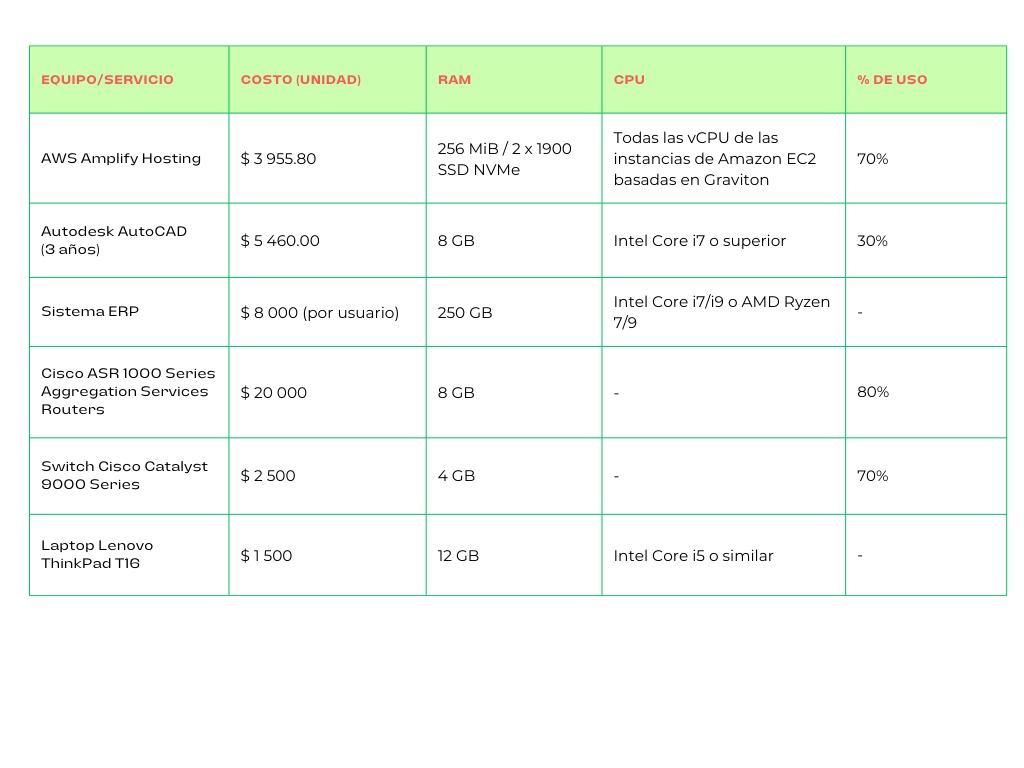
\includegraphics[width=0.8\textwidth]{cuadro_caloracion_capacidades_tic.jpeg}
        \caption{cuadro de la valoración de capacidades de las TIC's de Alicorp}
    \end{figure}

    \subsubsection{Requerimientos del negocio}
    Desarrollar una plataforma de gestión operativa y administrativa que abarque toda la cadena de valor, desde la producción hasta la distribución, asegurando la calidad en sus productos y precios competitivos en el mercado. 
    Crear y mantener alianzas con proveedores de materias primas, distribuidores y socios tecnológicos para fortalecer la cadena de suministro y mejorar la eficiencia operativa. 
    Fomentar una relación de confianza y lealtad con los clientes a través de programas de fidelización y atención personalizada que aborden sus necesidades de manera rápida y efectiva. 
    Optimizar la logística para garantizar una distribución eficiente y oportuna de los productos en los diferentes canales de venta, minimizando tiempos de entrega y costos operativos. 
    Mantener la seguridad y el buen funcionamiento de los sistemas operativos y la infraestructura tecnológica para asegurar la continuidad del negocio y una experiencia satisfactoria para los clientes. 
    Innovar continuamente en procesos de producción y soluciones tecnológicas para mejorar la competitividad y mantener la rentabilidad del negocio. 
    Asegurar el crecimiento sostenible y la generación de valor para los accionistas mediante una gestión eficiente de los recursos y el desarrollo de productos de alto valor agregado. 

    \subsubsection{Requerimientos de las TIC’s}
    Implementar soluciones tecnológicas que optimicen la gestión operativa y administrativa, garantizando la calidad y eficiencia en los procesos. 
    Mantener al personal capacitado y al tanto de nuevas tecnologías y actualizaciones en los procedimientos internos y externos. 
    Asegurar que las soluciones tecnológicas estén alineadas con los objetivos estratégicos de Alicorp y las necesidades específicas del sector de consumo masivo. 
    Evaluar e implementar tendencias tecnológicas que mejoren la competitividad de Alicorp, como la automatización en la producción, el uso de big data en la toma de decisiones y la integración de tecnologías IoT en la cadena de suministro. 
    
    \subsubsection{Proveedores }
    \paragraph*{Amazon Web Services (AWS)} Amazon Web Services (AWS) es una plataforma de servicios en la nube que ofrece una amplia gama de servicios y soluciones para ayudar a las empresas y desarrolladores a gestionar y escalar sus infraestructuras tecnológicas. 

    \paragraph*{Cisco} Cisco ofrece una amplia gama de servicios y soluciones para empresas, abarcando desde infraestructura de red y seguridad hasta colaboración y gestión de datos. 
    
    \paragraph*{Autodesk} Autodesk ofrece software y servicios diseñados para diseñar, ingeniería y construir y crear contenido digital. Sus soluciones están orientadas a una amplia gama de industrias, incluyendo arquitectura, ingeniería, construcción, manufactura, medios y entretenimiento. 
